% !TEX root = ../eval.tex

\section{Data}%
\label{sec:data}

\subsection{Dataset description}%
\label{sub:dataset_description}

I use data from Money Dashboard (MDB), a UK-based financial aggregation app
that allows users to link accounts from different banks to obtain an integrated
view of their finances in order to help them to reduce their spending and
increase their savings. Figure~\ref{fig:mdb} shows a screenshot from MDB's
website (left) and an example of its user interface (right). The complete
dataset contains more than 500 million transactions made between 2012 and June
2020 by about 270,000 users, and provides information such as date, amount, and
description of the transaction as well as account and user-level information.

\begin{figure}[h]
    \centering
    \caption{Money Dashboard website and user interface}%
    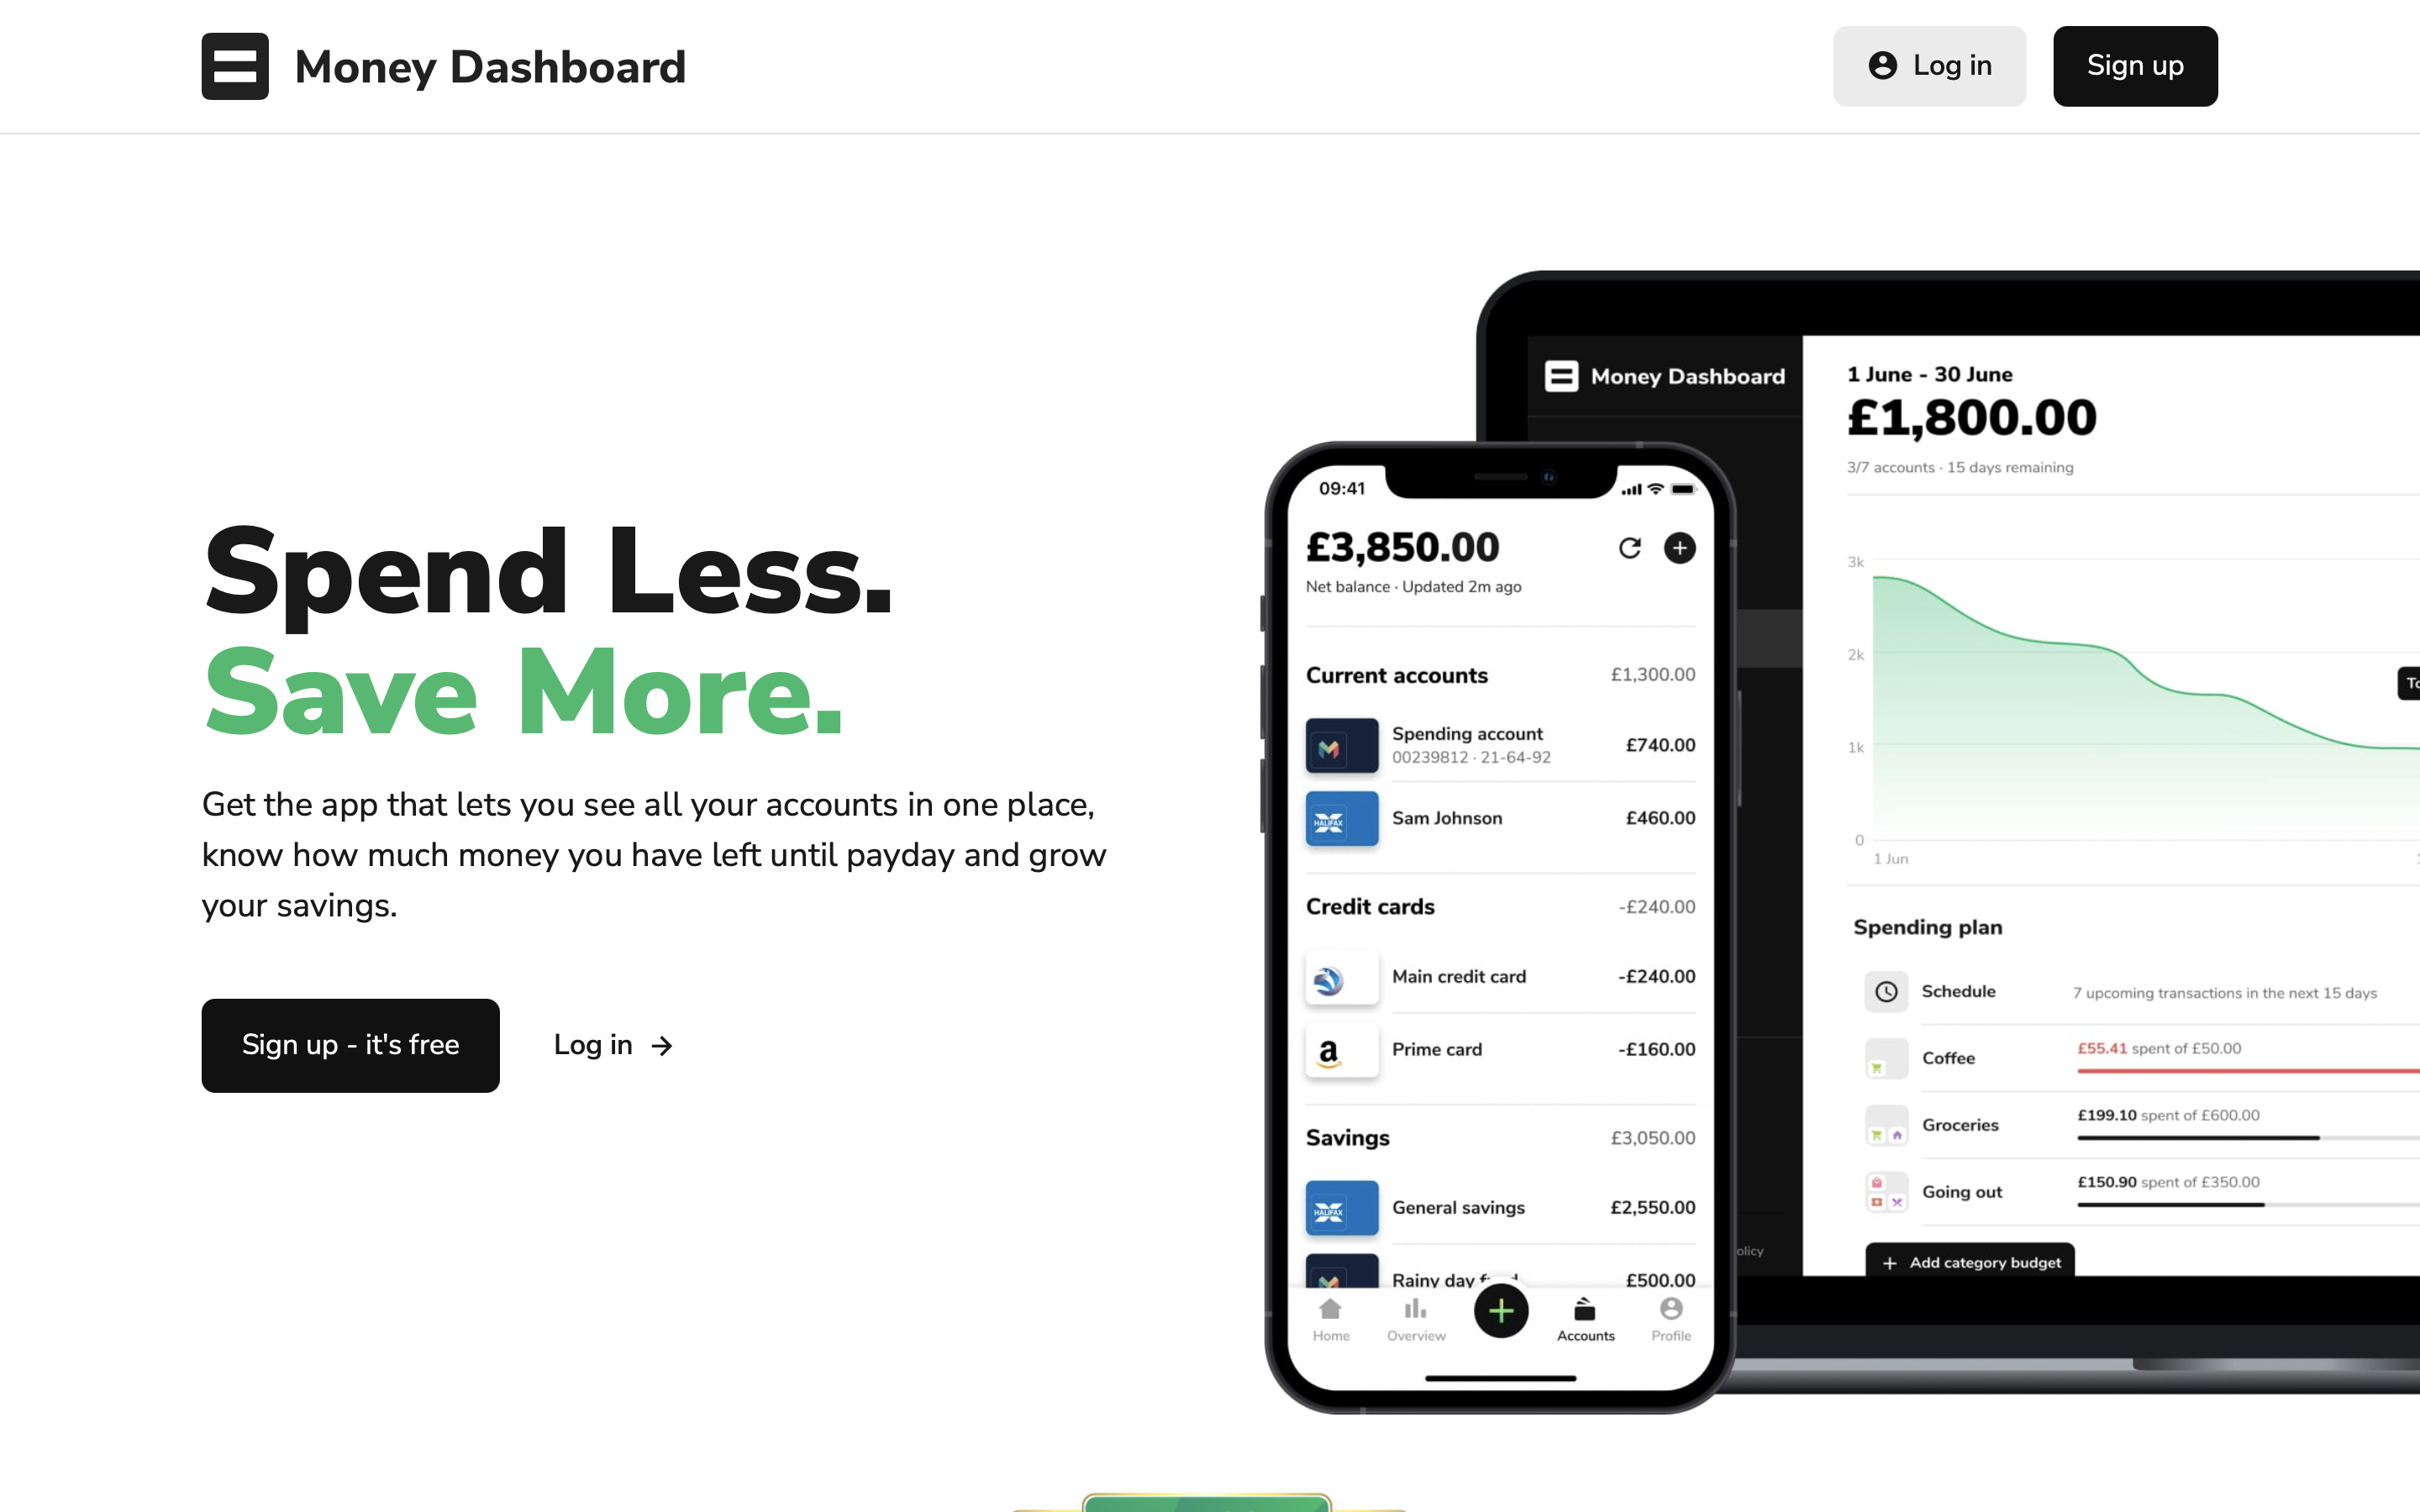
\includegraphics[width=0.49\linewidth]{\figdir/mdb_website}
    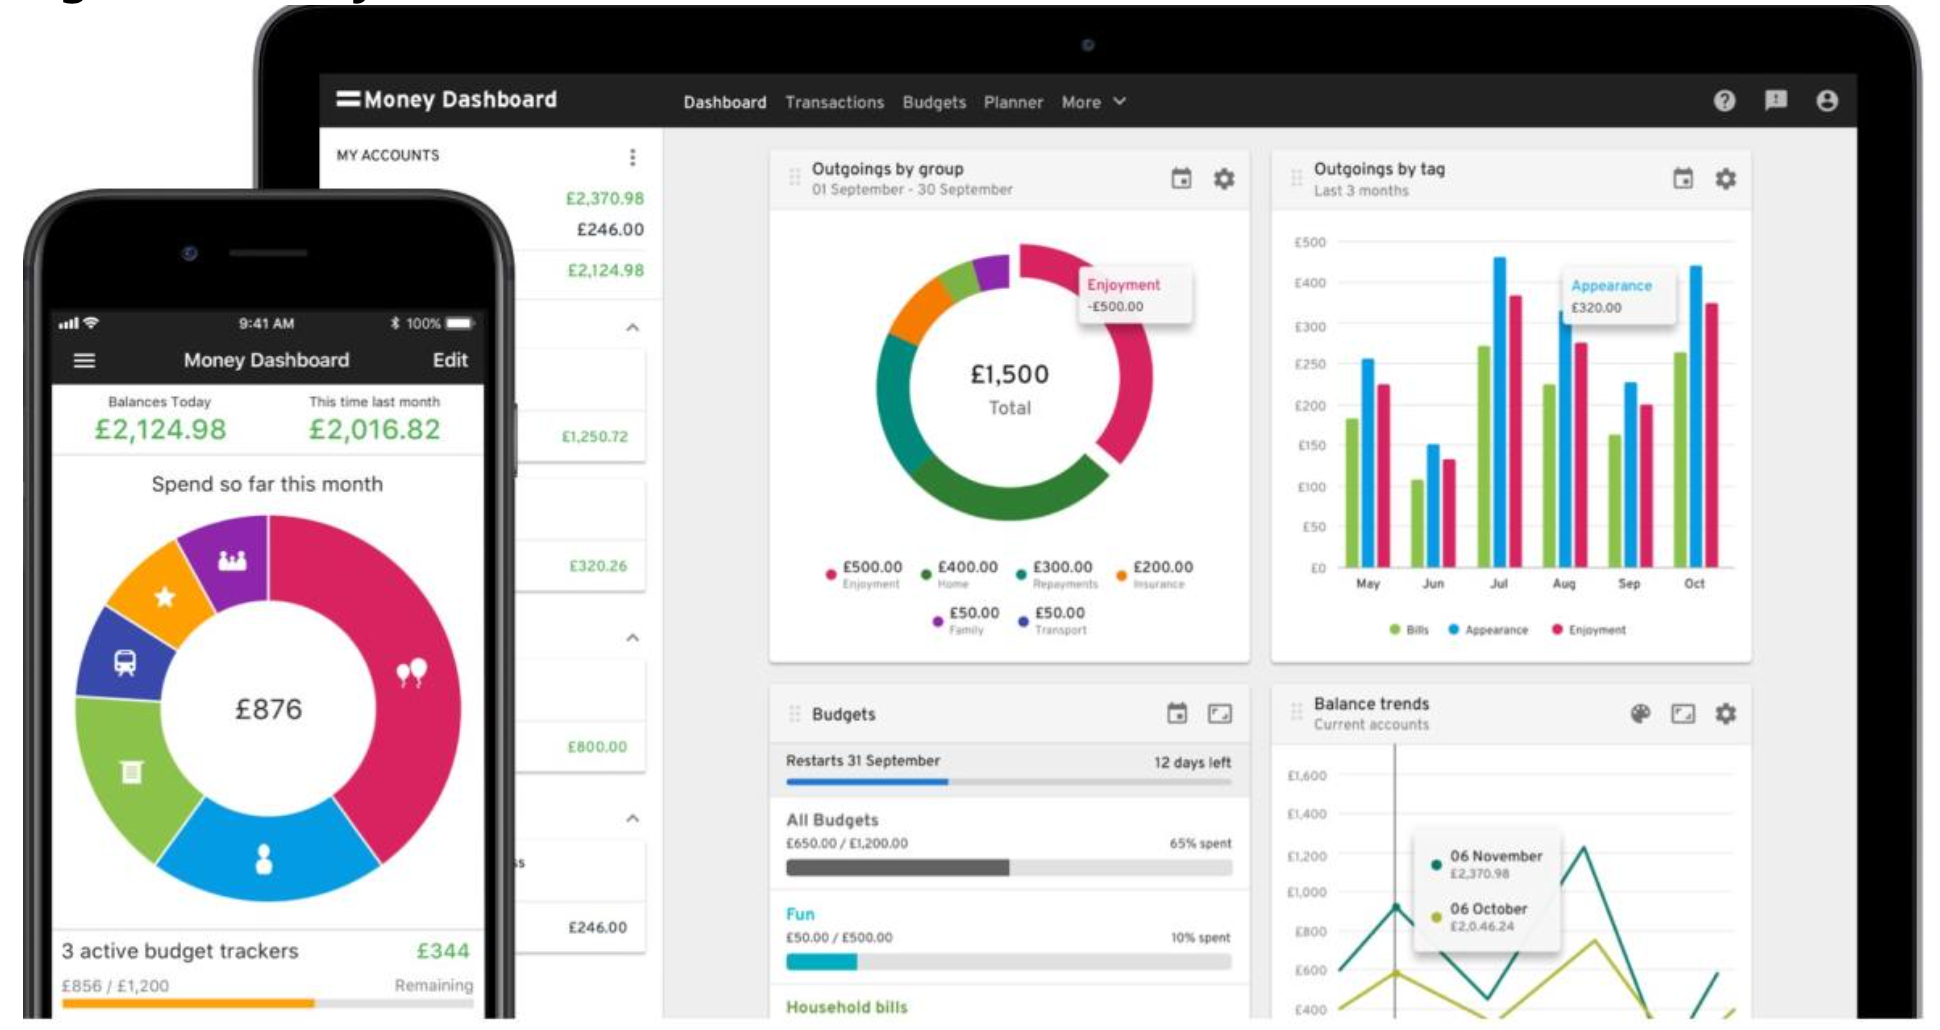
\includegraphics[width=0.49\linewidth]{\figdir/mdb_ui}
    \label{fig:mdb}
    \fignote{\textwidth}{Screenshot from the top of the Money Dashboard website
    (left) and example of its user interface (right), illustrating some of the
transaction grouping and budgeting functions.} 
\end{figure}

Crucially, for this paper, MDB can access up to three years of historic data
for each linked account. Figure~\ref{fig:treatplot} shows how we can leverage
pre-signup data provided in the MDB data to construct valid control groups.
Each row of cells shows data for one of 200 randomly selected users, with red
cells indicating data from pre-signup months and blue cells indicating data
from post-signup months. Signup thus occurred sometime during the first blue
coloured month, and we can use users who have not yet signed up (whose cells
are still red) as a comparison group. In my analysis below, I will use this
data structure to compare the outcomes of users who start using the Money
Dashboard app at a particular point in time with users who have not yet started
using the app at that time.

\begin{figure}[h]
\centering
\caption{Pre and post-signup data availability}%
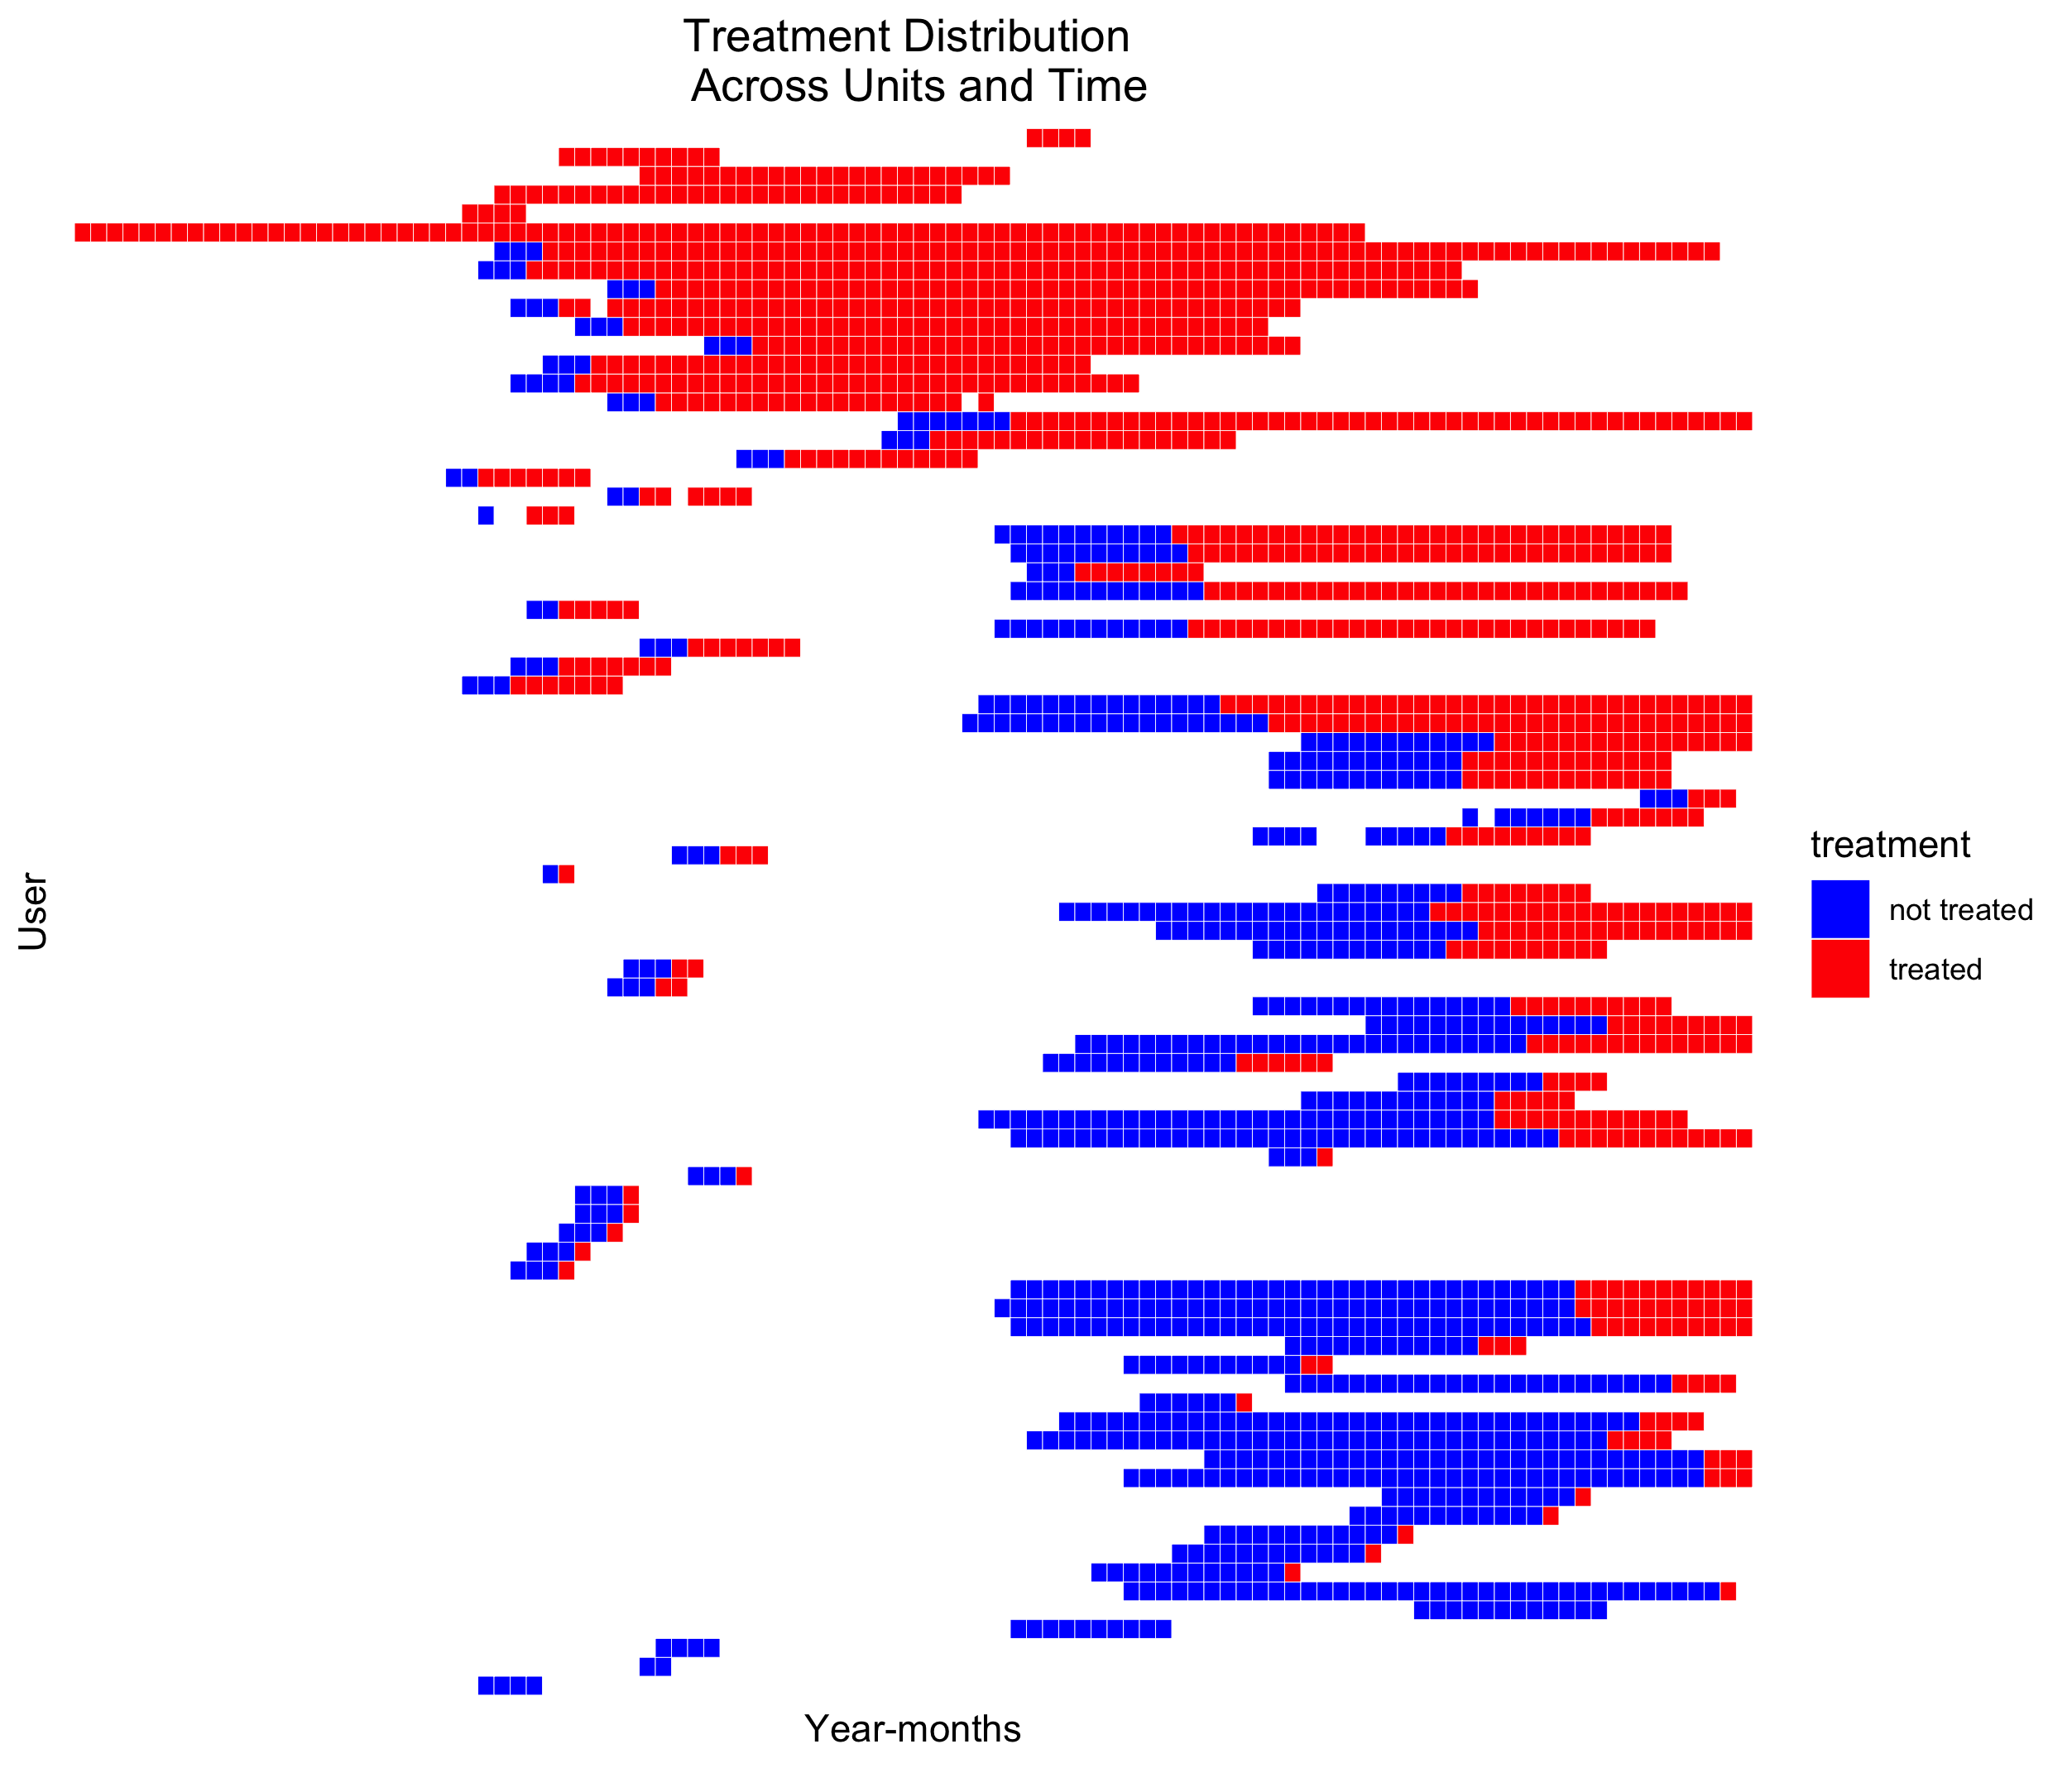
\includegraphics[width=0.8\linewidth]{\figdir/treatplot_sample_raw.png}
\label{fig:treatplot}
\fignote{\textwidth}{Each horizontal line shows the observed pre and post
    signup periods in blue and red, respectively, for one of 200 randomly
    selected users. The faint vertical white lines indicate month borders,
    whitespace indicates periods in which we do not observe users. To
the left of the observed period, this is because the app cannot access data
before that point; to the right, because they have
stopped using the app.}
\end{figure}

The data's main advantage for the study of consumer financial behaviour is that
it allows us to observe all savings and spending transactions for users who
linked all their financial accounts. This is important since it means that we
can be sure that any changes we observe in some of a user's account are not
offset by changes in unlinked accounts.\footnote{For an example where debt-reduction in
one set of accounts is offset by an increase in debt by another set of account,
see \citet{medina2021side}.} Furthermore, data is collected automatically and
in real-time rather than through surveys that collect data with a time-lag and
often rely on consumer's ability and willingness to provide accurate
information.

The data's main limitation is that because users's self select into using MDB,
the sample is not representative of the wider UK population: it is well
documented that FinTech app users are more likely to be male, younger, and
higher-income earners than the average person \citep{carlin2019generational}.
Also, as pointed out in \citet{gelman2014harnessing}, a willingness to share
financial information with a third party might not only select on demographic
characteristics, but also for an increased need for financial management or a
higher degree of financial sophistication. However, because, as discussed in
the introduction, the aim of this paper is to assess the effect of MDB on
people who choose to use it, the lack of representativeness is not an
issue.\footnote{For an example of how re-weighing can be used to mitigate the
non-representative issue, see \citet{bourquin2020effects}.} A second limitation
is that while we can observe user's complete financial behaviour if they add
all their financial accounts to the app, it is not trivial to distinguish
between users who do and do not do that. I address this challenge in the sample
selection process documented below. A third issue is that while the app is able
to classify many transactions into types, it misclassified some transactions
and cannot classify others altogether. I address this as part of the cleaning
process documented below.

\subsection{Preprocessing}%
\label{sub:preprocessing}

\paragraph{Data cleaning:}%
\label{par:data_cleaning}

I use the dataset described above for a number of projects, and perform a
number of steps to create a minimally cleaned version of the dataset that is
the basis for all such projects. These steps are performed in a dedicated data
repository and not run as part of this project.\footnote{The module with all
cleaning functions is available on
\href{https://github.com/fabiangunzinger/mdb_eval/blob/5f0346faf9b7058cd29fddd1c6ee9b0988b4fac6/src/data/clean.py}{Github}.}
Here, I briefly describe the main cleaning steps and their rationale. I drop
the fewer than 1 in 1000 transactions with a missing description string because
these cannot be categorised. I also group transactions into transfer, spend,
and income subgroups, following \citet{muggleton2020evidence} to define spend
subgroups and \citet{hacioglu2021distributional} to define income
subgroups.\footnote{ The precise list used to classify transactions is
available on
\href{https://github.com/fabiangunzinger/mdb_eval/blob/92af366d4c4052cc7a7f78a6178086de8ecdfb75/src/data/txn_classifications.py}{Github}.}
Finally, I classify as duplicates and drop transactions with identical user ID,
account ID, date, amount, and transaction description. This will drop some
genuine transactions, such as when a user buys two identical cups of coffees at
the same coffee shop on the same day. However, data inspection suggests that in
most cases, we remove genuine duplicates.

To minimise the influence of outliers, I winsorise all variables at the 1
percent level or -- if we winsorise on both ends of the distribution -- at the
0.5 percent level.\footnote{The code that performs the winsorisation are
    available on
\href{https://github.com/fabiangunzinger/mdb_eval/blob/d04fe186bb5cca884af2b7c1c7ad429674ef701d/src/data/transformers.py}{Github}.}
I rely on winsorisation (replacing top values with percentile values) instead
of trimming (replacing top values with missing values) because data inspection
suggests that in most cases, very large (absolute) values are not the result of
data errors, which would call for trimming, but reflect genuine outcomes, which
makes winsorising appropriate because it leaves these observations in the data
while lowering their leverage to influence results.


\paragraph{Sample selection:}%
\label{par:sample_selection_}

The three main goals of sample selection are to select a sample of users for
whom I can be reasonably certain to observe all relevant financial
accounts,\footnote{Relevant accounts include all current, savings, and
credit-card accounts, but exclude long-term savings and investment accounts.}
account histories of at least 12 months, and who are not using MDB for business
purposes. Table~\ref{tab:selection} lists the precise conditions I apply to
implement these criteria and their effect on sample size.\footnote{The code
that implements the selection criteria is available on
\href{https://github.com/fabiangunzinger/mdb_eval/blob/main/src/data/selectors.py}{Github}.}

In my main analysis, I show effects of app use for the 12-months period from 6
months before and 5 months after MDB signup, treating the month of signup as
period 0. To ensure that results are not affected by the number of accounts we
observe for an individual, it is thus critical that we can observe at least 12
months of history for all accounts a user adds to the platform. This ensures
that in the extreme case where a user adds an account they had used for some
time in the fifth month after they signed up, I observe all transactions on
that account throughout the 12-month period of interest. To see why this is
important, consider a user who has made monthly payments of \pounds100 into a
savings account for two years by the time they sign up to MDB but links that
account only five months after joining. In this case, we can only observe the
historical payments if MDB can access at least 12 months of history. If this
were not the case, and MDB can only, say, access 6 months of history, we would
erroneously conclude that the user started saving \pounds100 starting in the
month they signed up. Data exploration suggests that all major banks start
providing 12 months of historical data from April 2017 onwards, which is why
include only users who sign up after that data.\footnote{The Jupyter Notebook
containing the data exploration is available on
\href{https://github.com/fabiangunzinger/mdb_eval/blob/371493bd78870cab7a303edb70687287e5bca4a9/notebooks/available_account_history.ipynb}{Github}.}

To ensure that I can be reasonably certain to observe users who have added all
their financial accounts to the app, I restrict our sample to users with at
least one savings and current account, with an annual after-tax income of at
least \pounds5,000, and a minimum of 10 transactions and a spend of \pounds200
every month. To remove users who might use the app for business purposes, I
drop users with more than 10 active accounts in any given month.

Finally, I drop test users -- users who signed up to the app before it was
publicly available -- and users that are not of working age (younger than
18 or older than 65) because these groups might have objectives other than to
reduce spending and increase savings.\footnote{I cannot identify test users
    precisely, but drop users who signed up prior to or during 2011, the first
year the app was in operation.} And I retain only users for whom we can observe
the complete set of demographic covariates (gender, age, region) to ensure all
users can be used throughout the analysis. 

\begin{table}
\centering\footnotesize
\caption{Sample selection}\label{tab:selection}
\begin{tabular}{lrrrr}
\toprule
                                       &  Users & User-months &       Txns & Txns (m\pounds) \\
\midrule
                            Raw sample & 27,175 &     795,338 & 65,972,558 &          12,527 \\
             Drop first and last month & 26,565 &     741,170 & 64,157,932 &          12,179 \\
  At least 6 months of pre-signup data & 11,835 &     310,517 & 29,244,871 &           5,743 \\
 At least 6 months of post-signup data &  6,404 &     195,050 & 19,681,242 &           3,957 \\
          At least one current account &  5,833 &     178,845 & 18,257,300 &           3,738 \\
          At least one savings account &  4,506 &     138,181 & 14,485,916 &           3,133 \\
At least \pounds5,000 of annual income &  1,877 &      57,064 &  6,493,155 &           1,386 \\
           At least 10 txns each month &  1,686 &      51,190 &  5,935,336 &           1,262 \\
  At least \pounds200 of monthly spend &  1,478 &      44,641 &  5,333,532 &           1,135 \\
      Complete demographic information &  1,240 &      38,087 &  4,598,590 &             952 \\
                           Working age &  1,219 &      37,377 &  4,529,599 &             929 \\
                          Final sample &  1,219 &      37,377 &  4,529,599 &             929 \\
\bottomrule
\end{tabular}

\tabnote{.95\textwidth}{Number of users, user-months, transactions, and
transaction volume in millions of British Pounds left in our sample after each
sample selection step.}
\end{table}

These steps do impact the sample size significantly. In fact, while it is not
surprising that only considering users that signed up after March 2017 would
reduce the sample size considerably, the large reduction in users due to
requiring at least one savings account, an annual after-tax income of at least
\pounds5,000, and at least 10 monthly transactions are surprising, and suggest
that the raw dataset contains a large number of users that do not use Money
Dashboard as intended. The drastic effect of the selection procedure on sample
size also underlines how important careful sample selection is to ensure that
we can be reasonably sure to observe all relevant financial transactions for
all users in the sample, and thus to be confident that observed changes in
financial behaviour do not reflect a shift of transactions between observable
and unobservable accounts.


\subsection{Variable definitions}%

The main outcome variables in my analysis are \textit{discretionary spend} and
\textit{savings}.

\paragraph{Discretionary spend:} Discretionary spend aims to capture spend
transactions over which users have a lot of control. It is calculated solely
based on card transactions with cash transactions excluded. This is because
cash transactions are recorded in the MDB data as ATM withdrawals, and it is
impossible to know what these funds were used for. Furthermore, I do not
include gasoline expenses in discretionary spend because many people use their
car to commute to work so that it is unclear what proportion of these expenses
are discretionary. A list of transaction tags used to identify discretionary
spend transactions and the code used create the variable are available on
\href{https://github.com/fabiangunzinger/mdb_eval/blob/f31bfcd7a330188cdd27968d41957ebf5b454099/src/data/aggregators.py\#L389}{Github}.

\paragraph{Savings:} Savings are calculated as net-inflows into all of a user's
savings accounts that are linked to Money Dashboard. To capture only
user-generated savings-account flows and not interest payments and similar
automated transactions, I include only transaction with an absolute value of
\pounds5 or higher. The code used to calculate savings account flows is also
available on
\href{https://github.com/fabiangunzinger/mdb_eval/blob/f31bfcd7a330188cdd27968d41957ebf5b454099/src/data/aggregators.py#L89}{Github}.


\subsection{Summary statistics}%
\label{sub:summary_statistics}

Figure~\ref{fig:sample_description} provides a view of some salient sample
characteristics. Panels A and B show that while distributions of disposable
income and total spend in 2019 broadly mirror that of the ONS Living Cost and
Food Survey (LCFS) data, the MDB data tends to slightly underestimate incomes
and overestimate spending.\footnote{I accessed the LCFS data via the UK Data
Service at the following url:
\url{https://beta.ukdataservice.ac.uk/datacatalogue/studies/study?id=8686}.}
Given that our sample is likely biased towards high-earners, as discussed
above, we would expect both income and spend to be higher than in the LCFS. Two
likely caveats to the data probably create discrepancies relative to the LCFS
data. First, as discussed in Section~\ref{sub:preprocessing}, I drop
unclassified transactions from the data, which biases both income and spending
downwards (i.e. spending would probably be even higher compared to the LCFS).
Second, it is likely that it is more challenging to automatically classify
income transactions than spend transactions, which might create an additional
downward bias on the income distribution.\footnote{\citet{bourquin2020effects}
    present an alternative algorithm to identify income transactions and find
that this leads to higher estimated incomes. I do not use their algorithm
because I only use disposable income as a covariate to capture relative income
differences between users.} Panels C, D, and E show that, as discussed in
Section~\ref{sub:dataset_description}, the sample is skewed towards users that
are younger, male, and live in the South East. Finally, Panel D shows that most
users use transact with one or two accounts per month.

\begin{figure}[H]
    \centering
    \caption{Sample characteristics}
    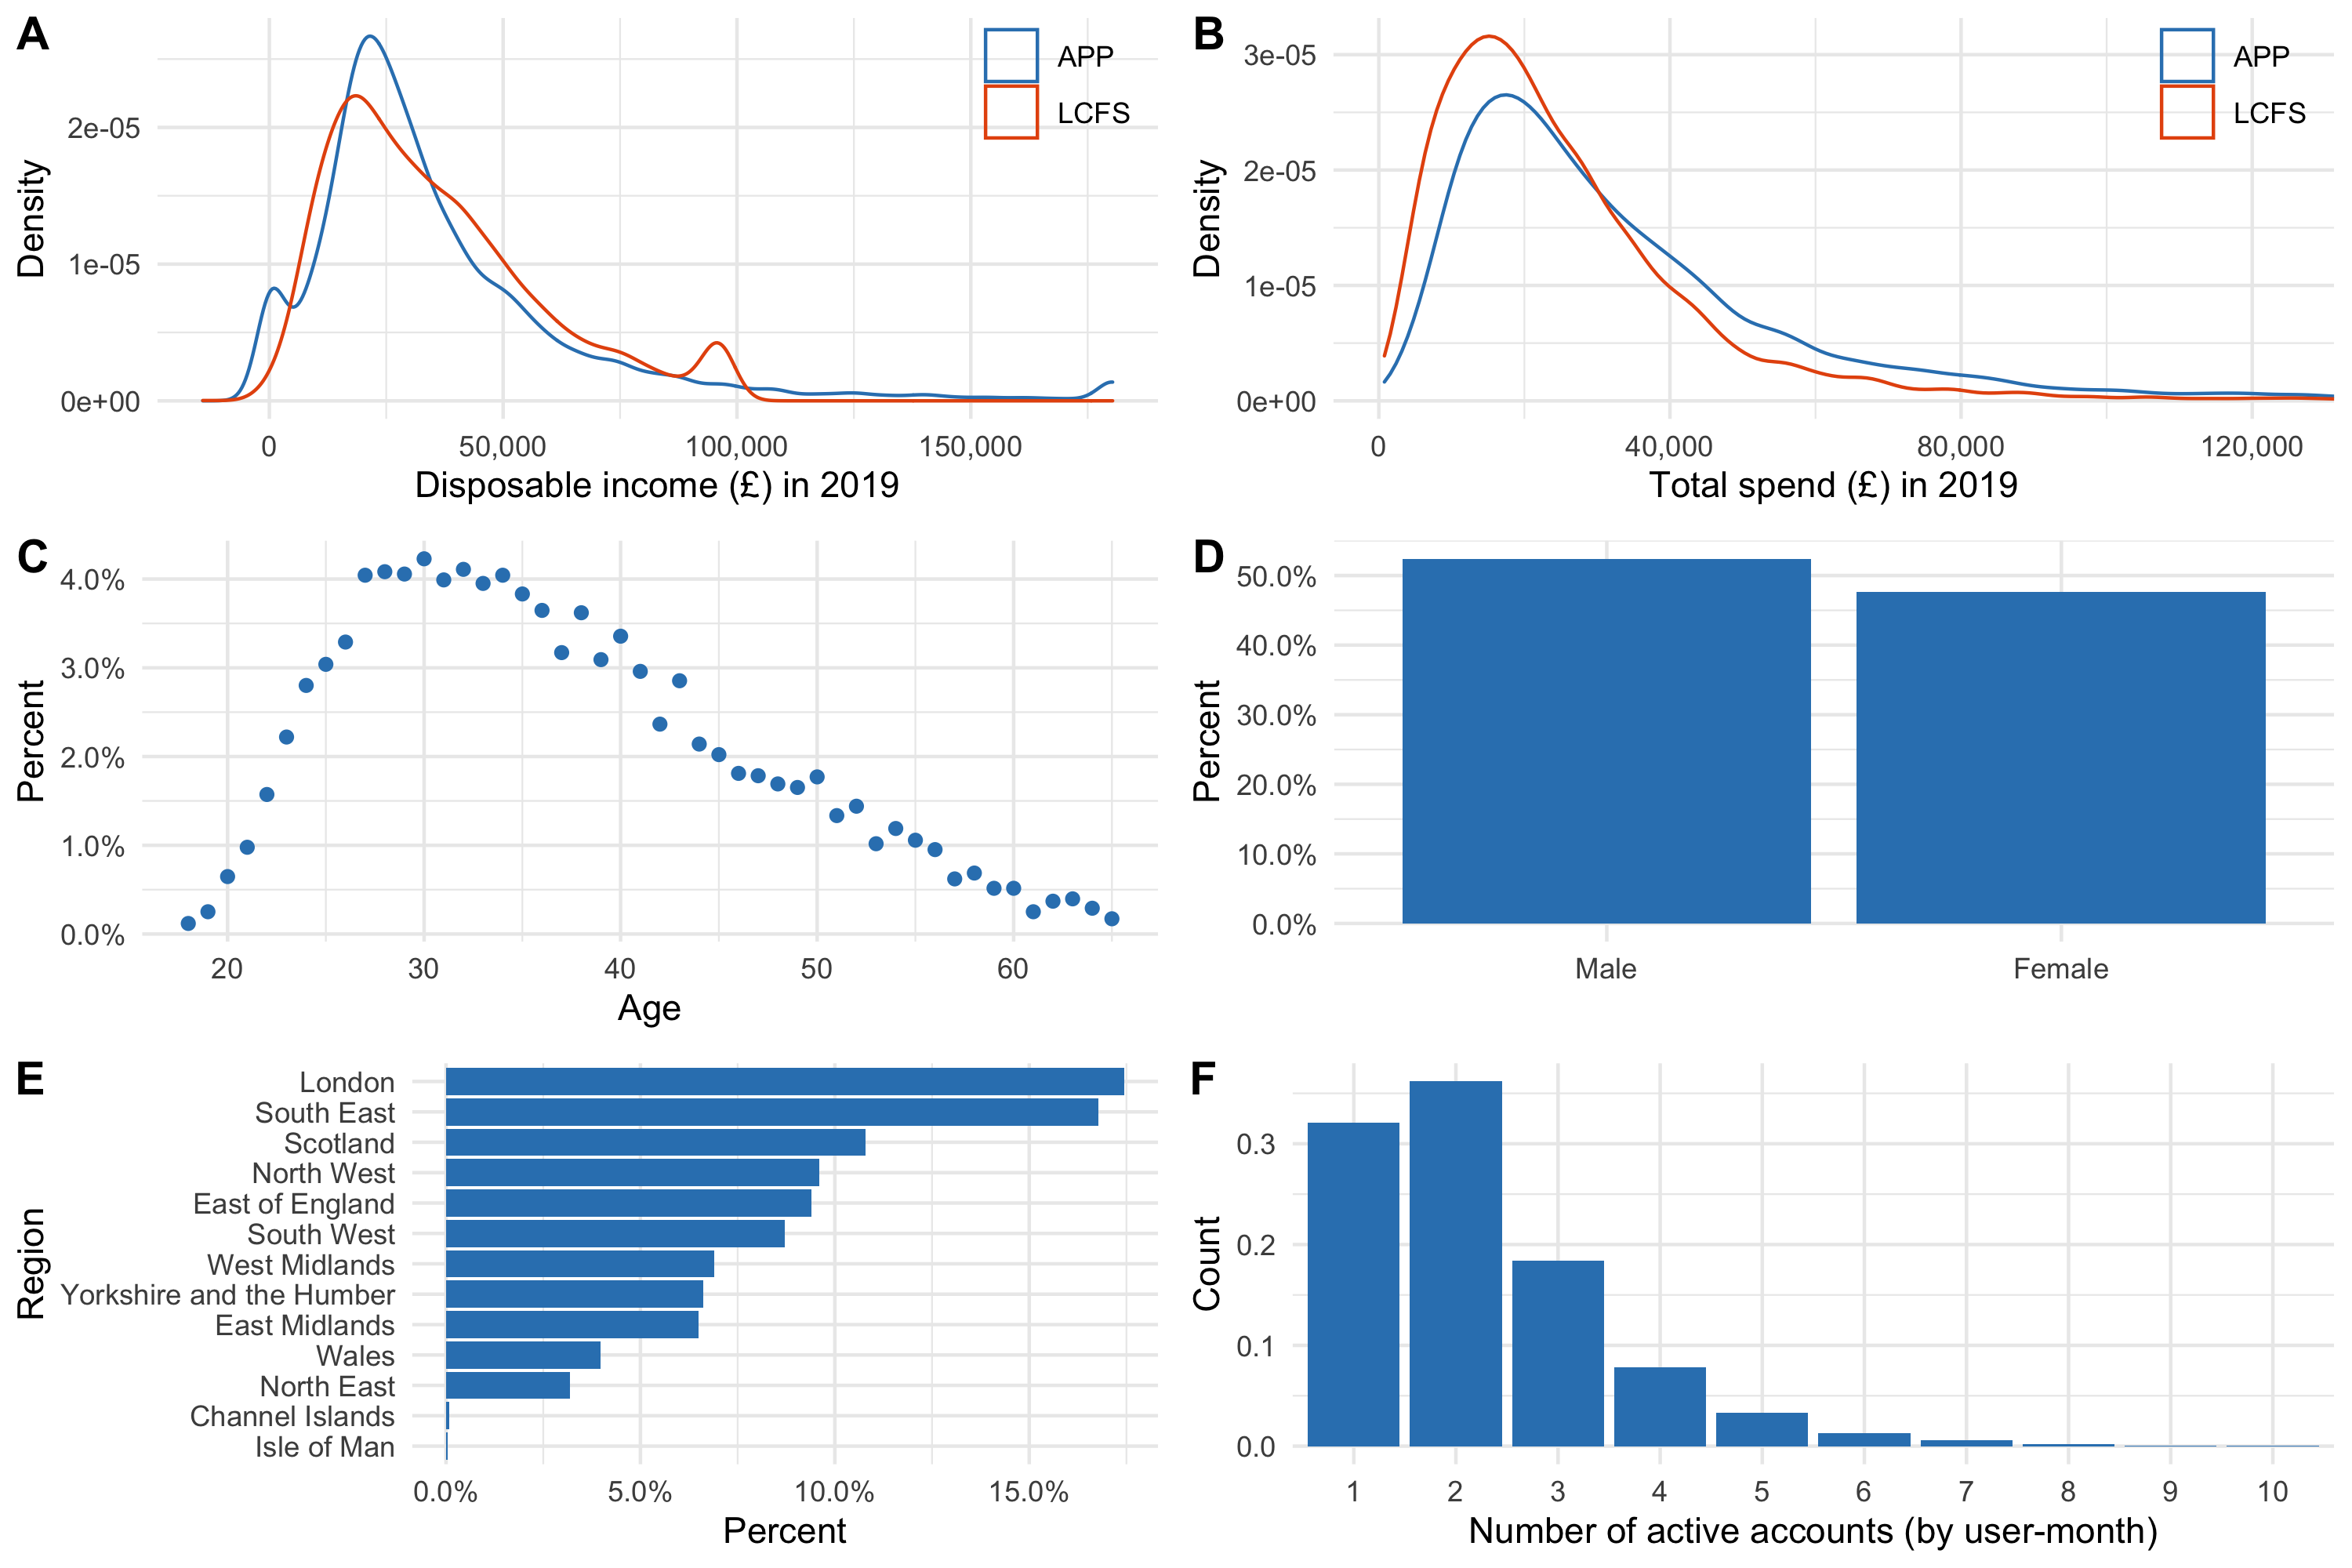
\includegraphics[width=\linewidth]{\figdir/sample_description.png}
    \label{fig:sample_description}
    \fignote{\textwidth}{Panels A and B show the distribution of disposable
        income and total spending in 2019, respectively, benchmarked against
        the 2018/19 wave of the ONS Living Cost and Food Survey (LCFS). The
        remaining panels show the data distributions of age, gender, region,
    and the number of active accounts.}%
\end{figure}

Table~\ref{tab:sumstats} provides additional summary statistics. It shows, for
instance, that the average number of monthly transactions is slightly above 100
(with a mean of 112 and a median of 101), that half of all user-month incomes
lie between \pounds1,407 and \pounds3,596, and that inflows into savings
accounts closely mirror outflows. It also suggests that discretionary
spend accounts for about 30 percent of total monthly spend

\begin{table}[ht]
\centering\tiny
\caption{Summary statistics}
\label{tab:sumstats}

\begin{table}[htbp]
   \centering
   \tiny
   \begin{threeparttable}[b]
      \caption{\label{tab:reg_compare} Regression results}
      \begin{tabular}{lcccccc}
         \tabularnewline \midrule \midrule
         Dependent Variable: & \multicolumn{6}{c}{Net-inflows}\\
         Model:                     & (1)                   & (2)                & (3)                & (4)                & (5)               & (6)\\  
         \midrule
         \emph{Variables}\\
         App use                    & 14.330$^{**}$         & 15.303$^{***}$     & 15.303$^{***}$     & 19.381$^{***}$     & 15.963$^{**}$     & 20.207$^{***}$\\   
                                    & [2.650; 26.009]       & [3.686; 26.919]    & [3.686; 26.919]    & [7.110; 31.652]    & [1.881; 30.045]   & [7.940; 32.473]\\   
         Month income               &                       & 0.053$^{***}$      & 0.053$^{***}$      & 0.060$^{***}$      & 0.053$^{***}$     & 0.058$^{***}$\\   
                                    &                       & [0.049; 0.058]     & [0.049; 0.058]     & [0.045; 0.075]     & [0.045; 0.060]    & [0.043; 0.073]\\   
         Month spend                &                       & -0.077$^{***}$     & -0.077$^{***}$     & -0.100$^{***}$     & -0.076$^{***}$    & -0.098$^{***}$\\   
                                    &                       & [-0.081; -0.073]   & [-0.081; -0.073]   & [-0.109; -0.091]   & [-0.091; -0.061]  & [-0.107; -0.089]\\   
         Disc. spend                &                       & 138.940$^{***}$    & 138.940$^{***}$    & 169.002$^{***}$    & 132.862$^{***}$   & 156.441$^{***}$\\   
                                    &                       & [115.597; 162.282] & [115.597; 162.282] & [128.874; 209.129] & [90.975; 174.750] & [115.907; 196.976]\\   
         Female                     &                       & -14.521$^{***}$    & -14.521$^{***}$    &                    & -14.247$^{***}$   &   \\   
                                    &                       & [-24.998; -4.044]  & [-24.998; -4.044]  &                    & [-21.206; -7.289] &   \\   
         Generation $=$ GenX        &                       & 39.071$^{***}$     & 39.071$^{***}$     &                    & 39.379$^{**}$     &   \\   
                                    &                       & [19.258; 58.885]   & [19.258; 58.885]   &                    & [9.611; 69.148]   &   \\   
         Generation $=$ Millennials &                       & 71.330$^{***}$     & 71.330$^{***}$     &                    & 71.699$^{***}$    &   \\   
                                    &                       & [51.964; 90.697]   & [51.964; 90.697]   &                    & [40.338; 103.060] &   \\   
         Generation $=$ GenZ        &                       & 42.302             & 42.302             &                    & 43.095$^{*}$      &   \\   
                                    &                       & [-9.381; 93.985]   & [-9.381; 93.985]   &                    & [-7.002; 93.192]  &   \\   
         Intercept                  & -20.523$^{***}$       & -59.208$^{***}$    & -59.208$^{***}$    &                    &                   &   \\   
                                    & [-30.679; -10.368]    & [-84.179; -34.237] & [-84.179; -34.237] &                    &                   &   \\   
         \midrule
         \emph{Fixed-effects}\\
         User FE                    &                       &                    &                    & Yes                &                   & Yes\\  
         Month FE                   &                       &                    &                    &                    & Yes               & Yes\\  
         \midrule
         \emph{Fit statistics}\\
         Observations               & 184,847               & 184,847            & 184,847            & 184,847            & 184,847           & 184,847\\  
         R$^2$                      & $3.13\times 10^{-5}$  & 0.01132            & 0.01132            & 0.10137            & 0.01203           & 0.10203\\  
         Within R$^2$               &                       &                    &                    & 0.00905            & 0.01117           & 0.00885\\  
         \midrule \midrule
         \multicolumn{7}{l}{\emph{Signif. Codes: ***: 0.01, **: 0.05, *: 0.1}}\\
      \end{tabular}
   \end{threeparttable}
\end{table}



\end{table}

